% file: 3-5-mst/bridge-spanning-tree.tex

\documentclass[tikz]{standalone}

\usetikzlibrary{chains}

\begin{document}

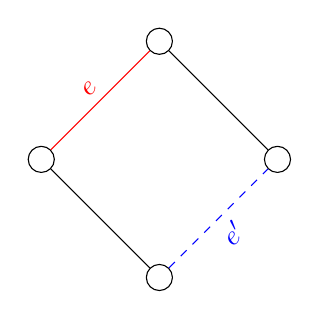
\begin{tikzpicture}[start chain=circle placed {at=(\tikzchaincount*90:1.5)},
  cnode/.style = {circle, draw, minimum size = 8pt}]
  \foreach \i in {1,...,4}
    \node [cnode, on chain] {};

  \path (circle-1) edge[red] node[sloped, above] {$e$} (circle-2)
	(circle-2) edge (circle-3)
	(circle-3) edge[dashed, blue] node[sloped, below] {$e'$} (circle-4)
	(circle-4) edge (circle-1);
\end{tikzpicture}
\end{document}

